\documentclass[a4paper,12pt,oneside]{book} % nie: report!


% pakiety
\usepackage{polski} % lepiej to zamiast babel!
\usepackage[utf8]{inputenc} % w razie kłopotów spróbować: \usepackage[utf8x]{inputenc}
\usepackage{fancyhdr} % nagłówki i stopki
\usepackage{indentfirst} % WAŻNE, MA BYĆ!
\usepackage[pdftex]{graphicx} % to do wstawiania rysunków
\usepackage{amsmath} % to do dodatkowych symboli, przydatne
\usepackage[pdftex,
            left=1in,right=1in,
            top=1in,bottom=1in]{geometry} % marginsy
\usepackage{amssymb} % to też do dodatkowych symboli, też przydatne
\usepackage{pdfpages}
\usepackage{lipsum}
\usepackage{multirow}
\usepackage{listings}
\usepackage{caption}
\usepackage{booktabs}
\usepackage{subcaption}
\usepackage{xcolor}
\graphicspath{ {./img/} }
\DeclareCaptionType{code}[Listing][Spis listingów] 

\definecolor{codegreen}{rgb}{0,0.6,0}
\definecolor{codegray}{rgb}{0.5,0.5,0.5}
\definecolor{codepurple}{rgb}{0.58,0,0.82}
\definecolor{backcolour}{rgb}{0.95,0.95,0.92}

\lstset{
	backgroundcolor=\color{backcolour},   
	commentstyle=\color{codegreen},
	keywordstyle=\color{magenta},
	numberstyle=\tiny\color{codegray},
	stringstyle=\color{codepurple},
	basicstyle=\ttfamily\footnotesize,
	breakatwhitespace=false,         
	breaklines=true,                 
	captionpos=b,                    
	keepspaces=true,                 
	numbers=left,                    
	numbersep=5pt,                  
	showspaces=false,                
	showstringspaces=false,
	showtabs=false,                  
	tabsize=2,
	float=h
}

% definicje nagłówków i stopek
\pagestyle{fancy}
\renewcommand{\chaptermark}[1]{\markboth{#1}{}}
\renewcommand{\sectionmark}[1]{\markright{\thesection\ #1}}
\fancyhf{}
\fancyhead[LE,RO]{\footnotesize\bfseries\thepage}
\fancyhead[LO]{\footnotesize\rightmark}
\fancyhead[RE]{\footnotesize\leftmark}
\renewcommand{\headrulewidth}{0.5pt}
\renewcommand{\footrulewidth}{0pt}
\addtolength{\headheight}{1.5pt}
\fancypagestyle{plain}{\fancyhead{}\cfoot{\footnotesize\bfseries\thepage}\renewcommand{\headrulewidth}{0pt}}


% interlinia
\linespread{1.25}


% treść
\begin{document}
\sloppy
\thispagestyle{empty}
\begin{titlepage}
	\begin{center}
		\vspace*{1cm}
		
		\Huge
		\textbf{Kompilacja Kernela Linux}
		
		\vspace{0.5cm}
		\LARGE
		Metoda stara i nowa
		
		\vspace{1.5cm}
		
		\textbf{Rafał Hrabia}\\
		\small nr indeksu 296583
		
		\vfill
		
		\vspace{0.8cm}
		
		\Large
		Informatyka I st.\\
		Uniwersytet Marii Curie-Skłodowskiej\\
		\today
		
	\end{center}
\end{titlepage}
\newpage{}

\thispagestyle{empty}
\newpage{}

\tableofcontents{}

\chapter{Przygotowanie}
\label{Przygotowanie}

W pierwszej kolejności po zalogowaniu się i przejściu do katalogu \emph{/usr/src} musimy zdobyć link do paczki z plikami źródłowymi kernela. Z racji tego, że
korzystam z wirtualnej maszyny bez interfejsu graficznego posłużę się komputerem, który hostuje maszynę wirtualną. Wchodzimy na stronę i przy użyciu menu
kontekstowego kopiujemy do schowka bezpośredni link to pliku(rys. \ref{link-copy}).

\begin{figure}[h]
	\centering
	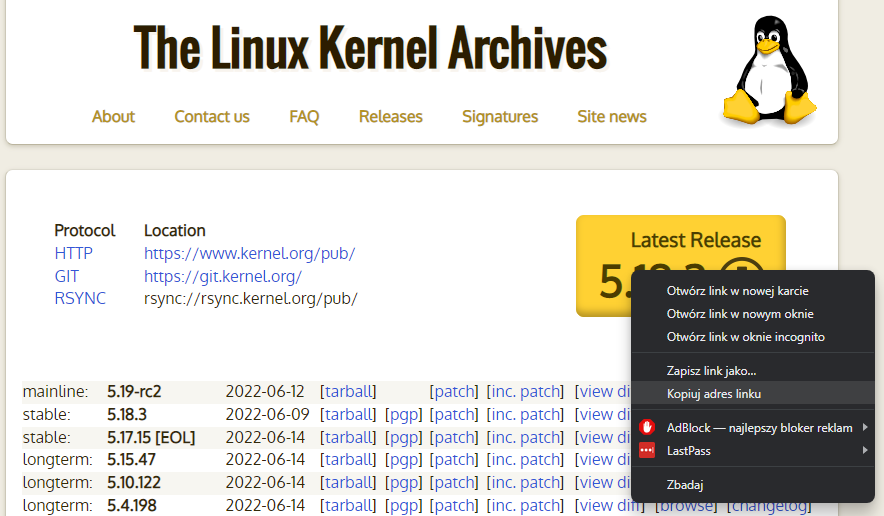
\includegraphics[scale=0.5]{01-link-copy.png}
	\caption{Kopiowanie linku}
	\label{link-copy}
\end{figure}

Do pobrania pliku jedynym słusznym wyborem będzie komenda \emph{wget}(rys. \ref{wget}).

\begin{figure}[h]
	\centering
	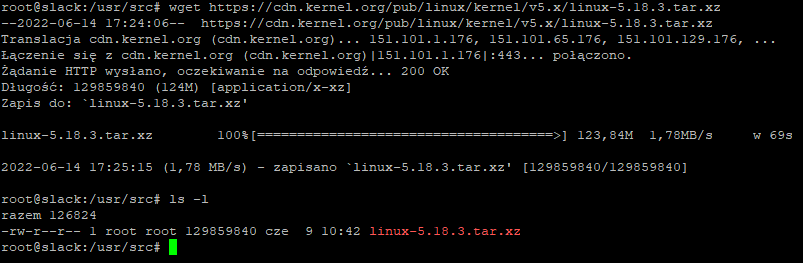
\includegraphics[scale=0.5]{02-wget}
	\caption{Pobieranie kernela}
	\label{wget}
\end{figure}

Jako, że pobrany plik jest to plik archiwum używamy na nim komendy \emph{tar -xvpf}(rys \ref{tar}).

Dla przypomnienia (flagi polecenia \emph{tar}):
\begin{itemize}
	\item x – wyodrębnia wymienione pliki
	\item v – wypisuje nazwy wszystkich plików
	\item f – określa nazwę pliku archiwum tar
	\item p - zachowuje ustawienia dostępu do plików
\end{itemize}

\begin{figure}[h]
	\centering
	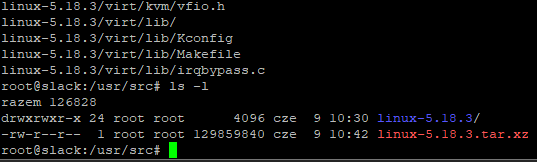
\includegraphics[scale=0.5]{03-tar}
	\caption{Rozpakowywanie archiwum}
	\label{tar}
\end{figure}

Jak można zauważyć został stworzony nowy folder zawierający pliki z archiwum.

Teraz musimy przekopiować \emph{config} znajdujący się w katalogu \emph{/proc} (rys \ref{config}). Ponieważ plik konfiguracji ma rozszerzenie wskazujące na to, że to archiwum gzip używamy polecenia \emph{zcat}.

\begin{figure}[h]
	\centering
	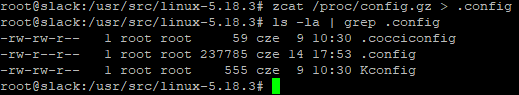
\includegraphics[scale=0.6]{04-config}
	\caption{Kopiowanie konfiguracji}
	\label{config}
\end{figure}

Przyda się zrobić kopię zapasową oryginalnego configu. W tym celu kopiujemy plik \emph{.config} do przykładowo pliku \emph{.config.bak} (rys. \ref{config-bak}).
\begin{figure}[h]
	\centering
	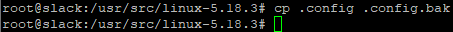
\includegraphics[scale=0.6]{05-config-bak}
	\caption{Kopia zapasowa}
	\label{config-bak}
\end{figure}

\chapter{Metoda stara}
\label{Metoda stara}

Przyszła pora na wywołanie polecenia \emph{make localmodconfig}. Po pomyślnym wykonaniu jesteśmy informowani o nadpisaniu konfiguracji do pliku \emph{.config} (rys. \ref{old-config}).

\begin{figure}[h]
	\centering
	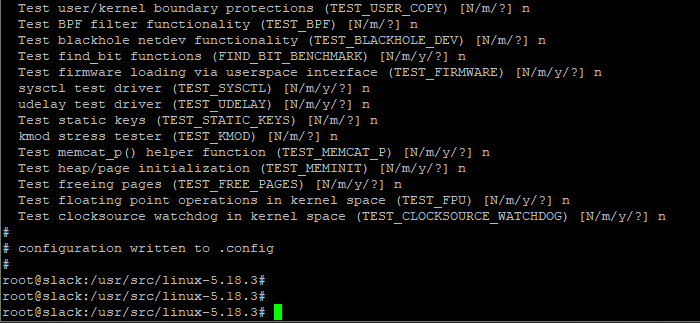
\includegraphics[scale=0.6]{06-old-config}
	\caption{Wynik polecenia \emph{make localmodconfig}}
	\label{old-config}
\end{figure}

Nastała wielka chwila - kompilacja jądra. W tym celu trzeba znowu użyć polecenia \emph{make}. Tym razem użyjemy parametru \emph{-j$<liczba>$} co pozwoli nam uruchomić kompilację kernela na wielu rdzeniach(lub wątkach?). W moim przypadku użyję liczby 8. 

\begin{figure}[h]
	\centering
	\includegraphics[scale=0.6]{08-bzimage}
	\caption{Kompilowanie kernela}
	\label{bzimage}
\end{figure}

\pagebreak

Kompilacja kernela przebiegła w zawrotnym czasie 4 minut i 45 sekund (mniej więcej).

\begin{figure}[h]
	\centering
	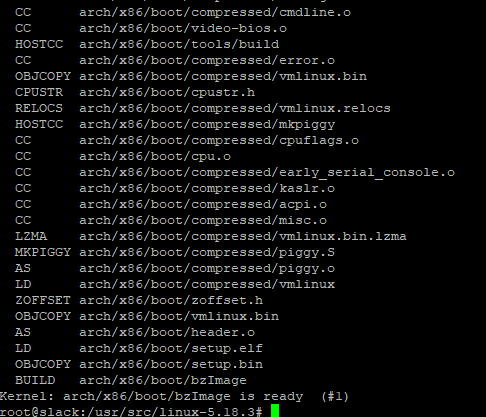
\includegraphics[scale=0.6]{09-compilation}
	\caption{Kompilowanie kernela - wynik}
	\label{compilation}
\end{figure}

Kompilację modułów zleca się również komendą make, ale zamieniamy parametr pozycyjny \emph{bzImage} na \emph{modules}.

\begin{figure}[h]
	\centering
	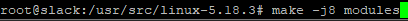
\includegraphics[scale=0.6]{10-modules}
	\caption{Kompilowanie modułów}
	\label{modules}
\end{figure}

Budowanie modułów zakończyło się zaskakująco szybko - w niecałe 36 sekund (tak, stałem ze stoperem w ręce). Pytanie czy tak powinno być? Czy to może zasługa Intel Core i9? Podejrzewam, że "stara metoda" ograniczyła ilość modułów do niezbędnego minimum. Przyjmijmy więc, że wszystko jest w porządku i kontynuujmy.

\begin{figure}[h]
	\centering
	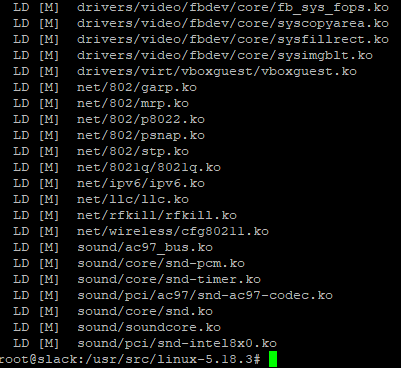
\includegraphics[scale=0.6]{11-modules-comp}
	\caption{Kompilowanie modułów - wynik}
	\label{modules-comp}
\end{figure}

\pagebreak

Instalacja modułów nie wprowadza nic nowego. Instalujemy moduły przy użyciu \emph{make}.

\begin{figure}[h]
	\centering
	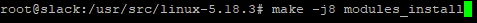
\includegraphics[scale=0.6]{12-modules-install}
	\caption{Instalowanie modułów}
	\label{modules-install}
\end{figure}

Bardzo szybkie 3 sekundy później (znowu mierzyłem) proces jest zakończony.

\begin{figure}[h]
	\centering
	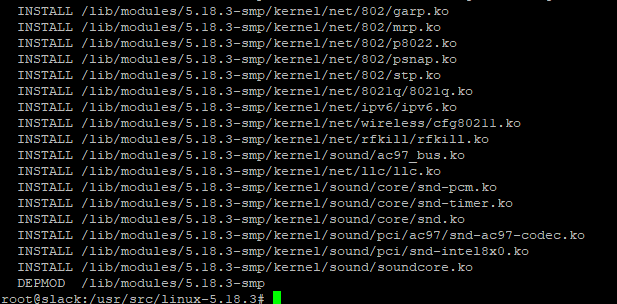
\includegraphics[scale=0.6]{13-modules-install-res}
	\caption{Instalowanie modułów - wynik}
	\label{modules-install-res}
\end{figure}

Możemy teraz przystąpić do kopiowania kernela do katalogu \emph{/boot}.

\begin{figure}[h]
	\centering
	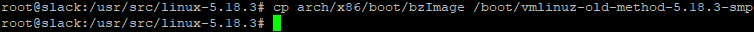
\includegraphics[scale=0.6]{14-bzimage-copy}
	\caption{Kopiowanie bzImage do katalogu /boot}
\end{figure}

\pagebreak

Plik jądra został z sukcesem przekopiowany do katalogu \emph{/boot}.

\begin{figure}[h]
	\centering
	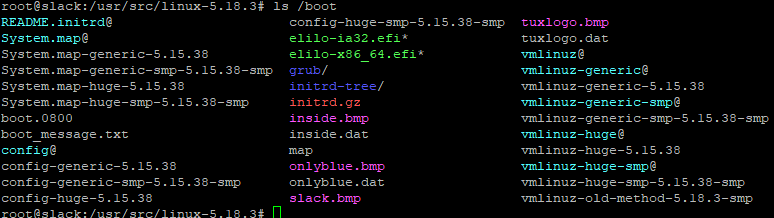
\includegraphics[scale=0.6]{15-boot}
	\caption{Kopiowanie bzImage do katalogu /boot - wynik}
\end{figure}

Musimy jeszcze przekopiować konfigurację i mapę systemu.

\begin{figure}[h]
	\centering
	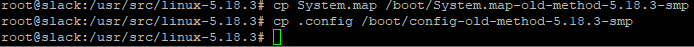
\includegraphics[scale=0.6]{16-config-copy}
	\caption{Kopiowanie configu i mapy symboli do katalogu /boot}
\end{figure}

Teraz możemy usunąć oryginalny plik \emph{System.map} i podłączyć skopiowany korzystając z linku symbolicznego.

\begin{figure}[h]
	\centering
	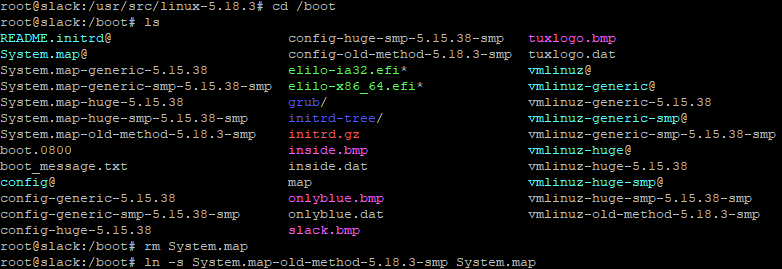
\includegraphics[scale=0.6]{17-system-map-link}
	\caption{Utworzenie linku symbolicznego do skopiowanej mapy symboli.}
\end{figure}

\pagebreak

Generujemy dysk startowy. Do wygenerowania polecenia używamy skryptu \emph{/usr/share/mkinitrd/mkinitrd\_command\_generator.sh}. Następnie wykonujemy wygenerowane polecenie.

\begin{figure}[h]
	\centering
	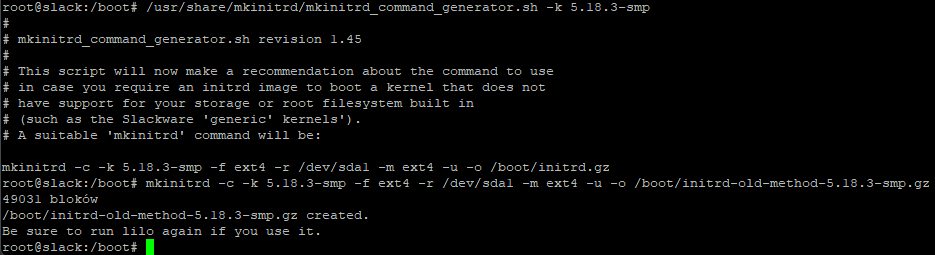
\includegraphics[scale=0.5]{23-ram-v2}
	\caption{Generujemy dysk ram}
\end{figure}

Pozostała nam już tylko konfiguracja lilo.

\begin{figure}[h]
	\centering
	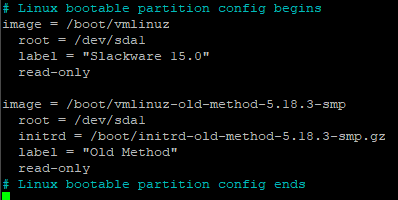
\includegraphics[scale=0.6]{19-lilo-conf}
	\caption{Konfiguracja lilo}
\end{figure}

\begin{figure}[h]
	\centering
	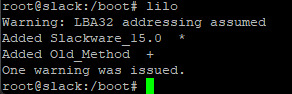
\includegraphics[scale=0.6]{24-lilo}
	\caption{Aktualizacja lilo}
\end{figure}

\pagebreak

Po uruchomieniu systemu widzimy nową pozycję "Old Method".

\begin{figure}[h]
	\centering
	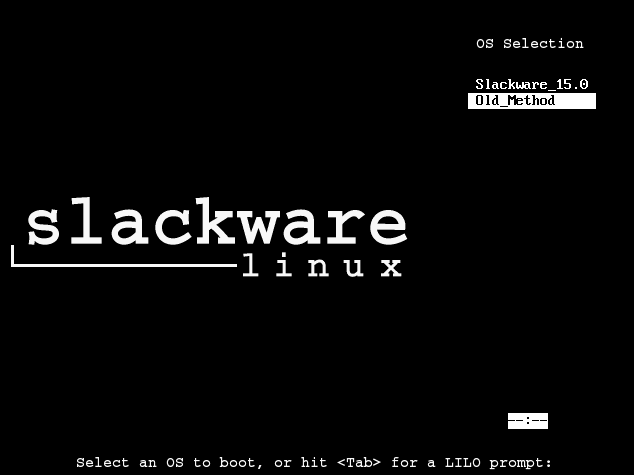
\includegraphics[scale=0.6]{25-lilo-view}
	\caption{Widok Lilo po uruchomieniu maszyny wirtualnej}
\end{figure}

Po chwili system się uruchamia i po zalogowaniu(lub nawet przed zalogowaniem) widzimy, że zmieniła się wersja jądra systemu.

\begin{figure}[h]
	\centering
	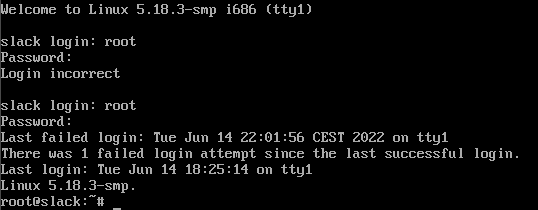
\includegraphics[scale=0.6]{26-success}
	\caption{Logowanie na root'a na nowym kernelu}
\end{figure}

Słowami zakończenia - nie obyło się bez błędów. Generując dysk ram za pierwszym razem przypadkowo nadpisałem oryginalny plik initrd.gz. Udało mi się sytuację prawdopodobnie uratować przekopiowując plik initrd.gz z poprzedniego snapshota, który utworzyłem, na maszynę, na której znajduje się Virtual Box, a następnie z powrotem na aktualną wersję systemu. Pomimo starań przy próbie odpalenia nowego kernela ten po długim czasie bootowania zaczął sypać błędami. Możliwe też, że to przez to, że przy tworzeniu dysku ram zapomniałem o dodaniu \emph{.gz} na końcu (lilo skonfigurowało się poprawnie i po uruchomieniu była widoczna nowa pozycja). Zauważyłem to już po fakcie. Stwierdziłem, że spróbuję jeszcze raz zaczynając od momentu kompilowania jądra. Za drugim razem poszło gładko i system wystartował. Nie umieszczam jeszcze raz zrzutów ekranu, gdzie treść w pierwszym i drugim podejściu była identyczna, żeby się nie powtarzać. 

\chapter{Metoda nowa}
\label{Metoda nowa}

Pracę nad nową metodą zaczynamy od przygotowania plików źródłowych i skopiowania configu. Teraz możemy stworzyć konfigurację systemu nową metodą.

\begin{figure}[h]
	\centering
	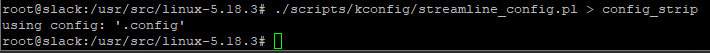
\includegraphics[scale=0.6]{28-config}
	\caption{Utworzenie configu nową metodą}
\end{figure}

Tak utworzony config-strip przekopiowujemy do .config i wywołujemy \emph{make oldconfig} zgodnie z instrukcją w skrypcie z poprzedniego zdjęcia.

\begin{figure}[h]
	\centering
	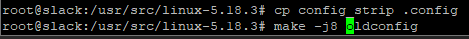
\includegraphics[scale=0.6]{29-config}
	\caption{Zmiana configu}
\end{figure}

\pagebreak

Teraz trzeba klikać Enter (i to dużo razy). W końcu gra w nie-czytanie-i-klikanie-enter się kończy i musimy przejść do następnego kroku.

\begin{figure}[h]
	\centering
	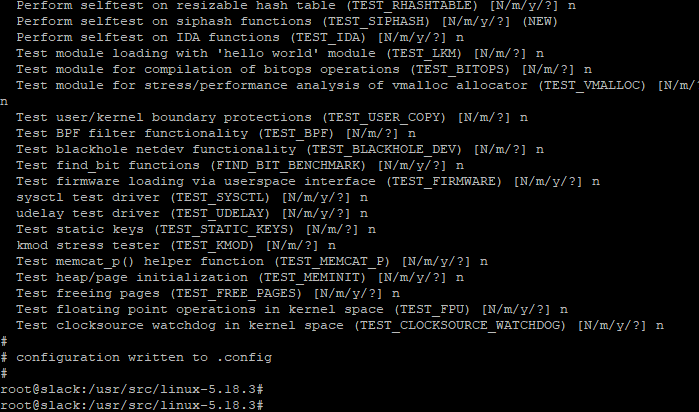
\includegraphics[scale=0.6]{30-config}
	\caption{Maraton klikania Enter}
\end{figure}

Kompilujemy jądro.

\begin{figure}[h]
	\centering
	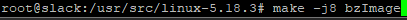
\includegraphics[scale=0.6]{31-comp}
	\caption{Kompilacja jądra}
\end{figure}

\begin{figure}[h]
	\centering
	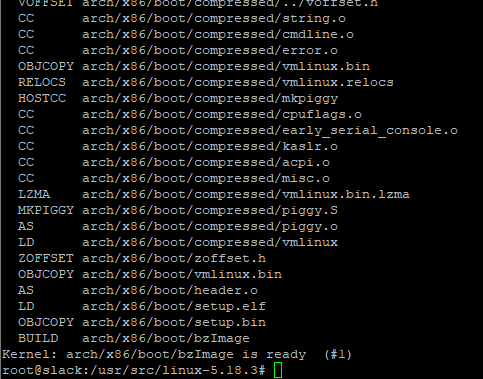
\includegraphics[scale=0.6]{32-comp}
	\caption{Kompilacja jądra - wynik}
\end{figure}

\pagebreak

Przechodzimy do kompilacji modułów.

\begin{figure}[h]
	\centering
	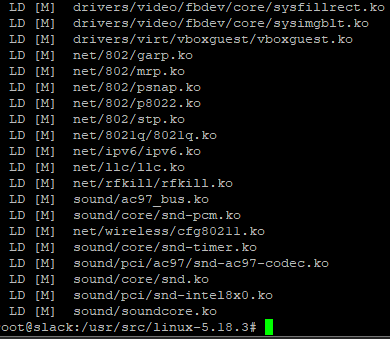
\includegraphics[scale=0.6]{33-comp}
	\caption{Kompilacja modułów - wynik}
\end{figure}

A następnie do instalacji modułów.

\begin{figure}[h]
	\centering
	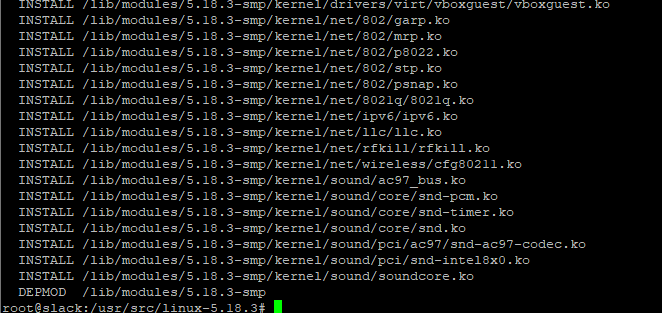
\includegraphics[scale=0.6]{34-install}
	\caption{Instalacja modułów - wynik}
\end{figure}

Kopiujemy niezbędne pliki.

\begin{figure}[h]
	\centering
	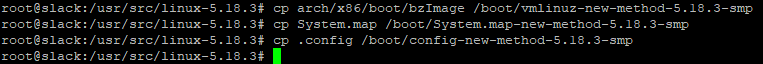
\includegraphics[scale=0.6]{35-copy}
	\caption{Kopiowanie plików}
\end{figure}

\pagebreak

Tworzymy link symboliczny do System.map.

\begin{figure}[h]
	\centering
	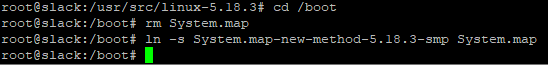
\includegraphics[scale=0.6]{36-sysmap}
	\caption{Utworzenie linku symbolicznego}
\end{figure}

Tworzymy dysk ram.

\begin{figure}[h]
	\centering
	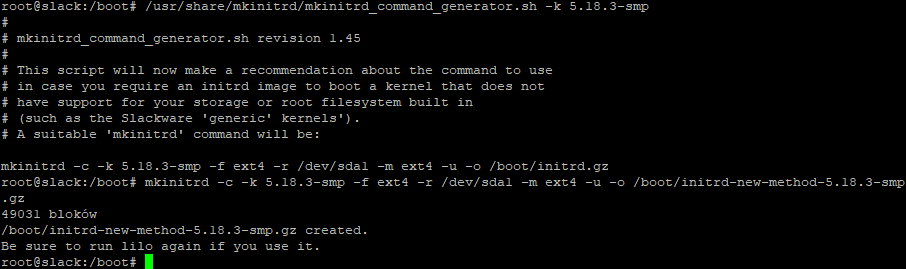
\includegraphics[scale=0.6]{37-ram}
	\caption{Stworzenie dysku ram}
\end{figure}

Konfigurujemy lilo.

\begin{figure}[h]
	\centering
	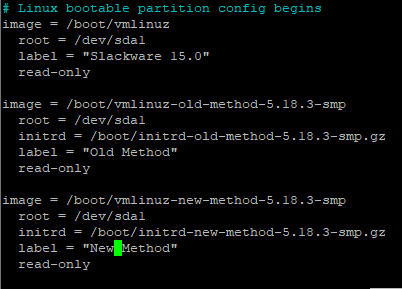
\includegraphics[scale=0.6]{38-lilo}
	\caption{/etc/lilo.conf}
\end{figure}

\pagebreak

I ponownie aktualizujemy

\begin{figure}[h]
	\centering
	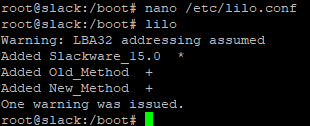
\includegraphics[scale=0.6]{39-lilo}
	\caption{Wynik komendy lilo}
\end{figure}

Po ponownym uruchomieniu maszyny mamy kolejną pozycję do wyboru.

\begin{figure}[h]
	\centering
	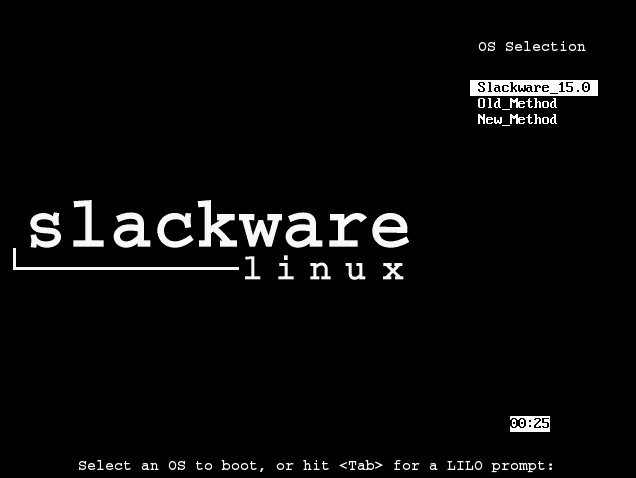
\includegraphics[scale=0.6]{40-lilo}
	\caption{Wynik komendy lilo}
\end{figure}

Widzimy, że zmieniła się wersja jądra.

\begin{figure}[h]
	\centering
	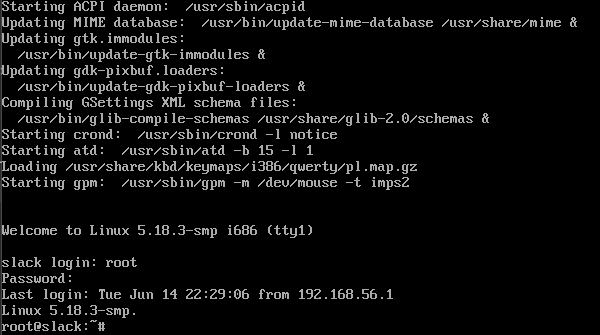
\includegraphics[scale=0.5]{41-root}
	\caption{Logowanie na root'a}
\end{figure}

\chapter{Wnioski}
\label{Wnioski}

Jak można się przekonać wykonując ćwiczenie - kompilacja kernela nie jest trudna, a jest nawet przyjemna. Przede wszystkim trzeba uważać na błędy ludzkie, takie jak złe nazwanie pliku i wykasowanie lub nadpisanie czegoś przez przypadek. Zdarza się. Oczywiście lekcja jest taka, że backupów nigdy za wiele. 

\end{document}
